\documentclass{article}
\usepackage[utf8]{inputenc}
\usepackage{blindtext}
\usepackage{amsmath, amsfonts, amsthm, centernot, enumerate}
\usepackage{geometry}
\usepackage{fancyhdr}
\usepackage{graphicx}

\geometry{a4paper,
left=30mm,
right=30mm,
top=15mm}
\linespread{1.2}
\setlength{\headheight}{24.0pt}

\renewcommand{\labelenumi}{(\alph{enumi})}

\newcommand{\N}{{\mathbb N}}
\newcommand{\Z}{{\mathbb Z}}
\newcommand{\Q}{{\mathbb Q}}
\newcommand{\R}{{\mathbb R}}
\newcommand{\C}{{\mathbb C}}

\newcommand{\ep}{{\varepsilon}}

\renewcommand{\P}{{\mathbb P}}
\newcommand{\E}{{\mathbb E}}
\newcommand{\I}{{\mathbb I}}

\DeclareMathAlphabet\mathbfcal{OMS}{cmsy}{b}{n}

\newtheoremstyle{break}
{\topsep}{\topsep}%
{\upshape}{}%
{\bfseries}{}%
{\newline}{}%
\theoremstyle{break}
\newcommand{\problem}[2]{\theoremstyle{break} \newtheorem*{thm#1}{#1}\begin{thm#1}#2\end{thm#1}}

\begin{document}
\problem{The Problem}{Let $X_1,\dots,X_n$ be independent and identically distributed (iid) for some distribution with parameter $\theta$. An estimator
$\hat{\theta}$ of parameter $\theta$ is said to be consistent if \[\lim_{n\to\infty}\P(|\hat{\theta}-\theta|\geq
\ep)=0\quad\text{or equivalently}\quad \lim_{n\to\infty}\P(|\hat{\theta}-\theta|\leq \ep)=1,\] for all $\ep>0$. Intuitively what
this means is that as the sample size increases, the probability that the estimator is the different from the true parameter tends
towards $0$. Or equivalently the probability that the estimator is the same as the true parameter tends to $1$.

Let $Y_1,\dots,Y_n$ be iid and $Y_i\sim\text{Expon}\left(1/\lambda\right)$. Consider the estimators of $\lambda$: $\tilde{\lambda}_1=1/n\sum_{i=1}^n Y_i$
and $\tilde{\lambda}_2=n\min\{Y_1,\dots,Y_n\}$. }
\medskip
\problem{The Analysis}{It can be shown (although we won't) that both $\tilde{\lambda}_1$ and $\tilde{\lambda}_2$ are unbiased. That is, $\E(\tilde{\lambda}_1)=
\lambda=\E(\tilde{\lambda}_2).$

\bigskip

To see that $\tilde{\lambda}_1$ is consistent, we can first calculate $\text{Var}(\tilde{\lambda}_1)=\lambda^2/n$, and then
use Chebyshev's Inequality to obtain 
\[\P(|\tilde{\lambda}_1-\E(\tilde{\lambda}_1)|\geq\ep)\leq\text{Var}(\tilde{\lambda}_1)/\ep^2 \implies
\P(|\tilde{\lambda}_1-\lambda|\geq\ep)\leq \lambda^2/n\ep^2.\] Thus by taking the limit as $n\to\infty$ of both sides we obtain
\[\lim_{n\to\infty}\P(|\tilde{\lambda}_1-\lambda|\geq\ep)\leq 0\implies\lim_{n\to\infty}\P(|\tilde{\lambda}_1-\lambda|\geq\ep)
=0,\] since probability is non-negative.

\bigskip

To see that $\tilde{\lambda}_2$ is inconsistent, notice that \[\lim_{n\to\infty}\P(|\tilde{\lambda}_2-\lambda|\geq \ep)=0\iff
\lim_{n\to\infty}\P(|\tilde{\lambda}_2-\lambda|^2\geq \ep^2)=0.\] Thus we need only find some $\ep>0$ for which
$\lim_{n\to\infty}\P(|\tilde{\lambda}_2-\lambda|^2\geq \ep^2)\neq0$. It can be shown that
$\text{Var}(\tilde{\lambda}_2)=\lambda^2$ We define a new random variable $Z_n=|\tilde{\lambda}_2-\lambda|^2=
(\tilde{\lambda}_2-\lambda)^2$, and we see $\E(Z_n)=\text{Var}(\tilde{\lambda}_2)= \lambda^2\centernot{\xrightarrow[n\to\infty]{}}
0$. Since $Z_n$ is positive, so is its expectation. Thus $\E(Z_n)$ is bounded below by some $\delta^2>0$. Now notice that the
expectation of $Z_n$ is bounded above by the maximum of the image of $Z_n$. Thus there must exist at least one element in the
sample space of $Z_n$ (namely the element that maximizes $Z_n$) such that $Z_n \geq \delta^2$. Therefore $\P(Z_n\geq
\delta^2)=\P(|\tilde{\lambda}_2-\lambda|^2\geq \delta^2)\neq 0$. In this limit this remains true. Thus
$\lim_{n\to\infty}\P(|\tilde{\lambda}_2-\lambda|^2\geq \ep^2)=0$ is not true for all $\ep>0$ (take $\ep=\delta$ as a counter
example). Therefore $\tilde{\lambda}_2$ is inconsistent.


}
\medskip
\problem{The Simulation}{While the analysis may be correct, it is not particularly convincing unless one is familiar with the probability theory. This is
where the simulation is helpful. By generating $1000$ samples of sizes from $n=1$ to $n=1000$, we can calculate the proportion of
samples for which the estimator was ``within $\ep$'' of the true parameter. By then plotting this proportion against sample size
we should see convergence for $\tilde{\lambda}_1$ but no convergence for $\tilde{\lambda}_2$. Note that I chose a small value of
$\lambda$ for my true parameter so that it converged more quickly and my laptop could finish the simulation. Indeed as $n$ gets
larger, the proportion of $\tilde{\lambda}_1$ that is ``within $\ep$'' of $\lambda$ is close to $1$. But the proportion of
$\tilde{\lambda}_2$ that is ``within $\ep$'' of $\lambda$ does not converge to anything.

\begin{center}
	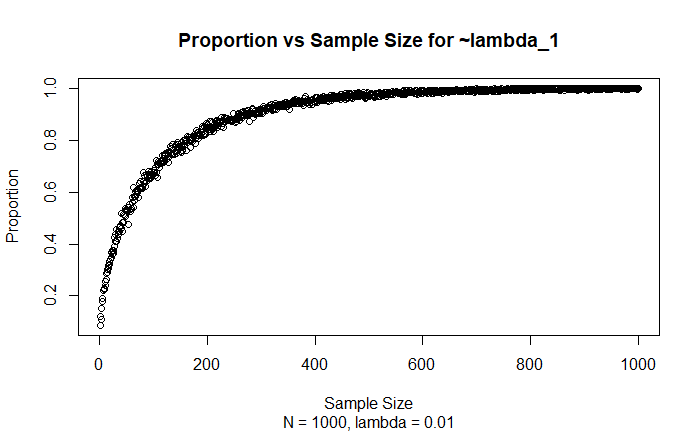
\includegraphics[scale=0.8]{proportion_plot_lambda_1.png}
	
	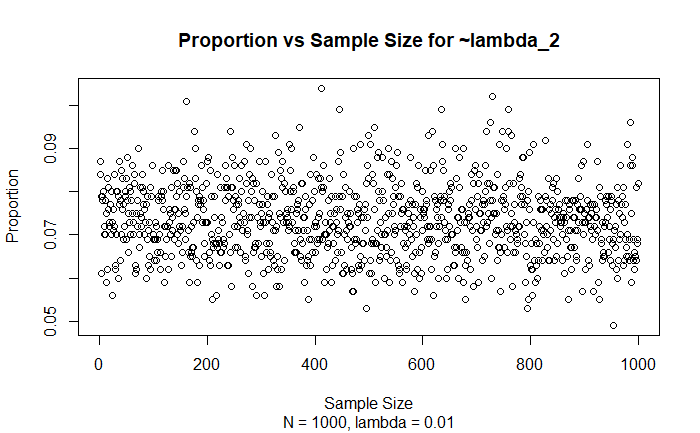
\includegraphics[scale=0.8]{proportion_plot_lambda_2.png}
\end{center}
}

\end{document}